
Online DQM applications are operated on the cms-cluster at P5 on event data. 
DQM distributions are created at two different levels:

\begin{enumerate}
\item {\bf DQM Sources in the HLT Filter Units:} \\
A limited number of histograms, as implemented in analyzer modules, can be processed at the level of the HLT where events are available at a rate of up to 100 kHz. The histograms (as stored in monitoring elements (ME)) are shipped out from the HLT filter units to the Storage Managers at the end of each luminosity section. Identical histograms from different filter units are summed up and sent to the SMProxyServer, a single access point, which provides access to the ME through a DQM histogram server to consumer applications. The SMProxyServer also saves the DQM histograms to files. 
\item {\bf DQM Sources operating off the Storage Manager Event Server:} \\
The Storage Manager Proxy Server also provides an event server which delivers events at the rate of order 10-15 Hz to event consumer applications. The events available events are part of special DQM stream the contents and selection are specified by the DQM group as part of the HLT configuration. 
\end{enumerate}
The storagemanager system is sketched in Fig.~\ref{fig:sm}.

\begin{figure}[!htbp]
\begin{center}
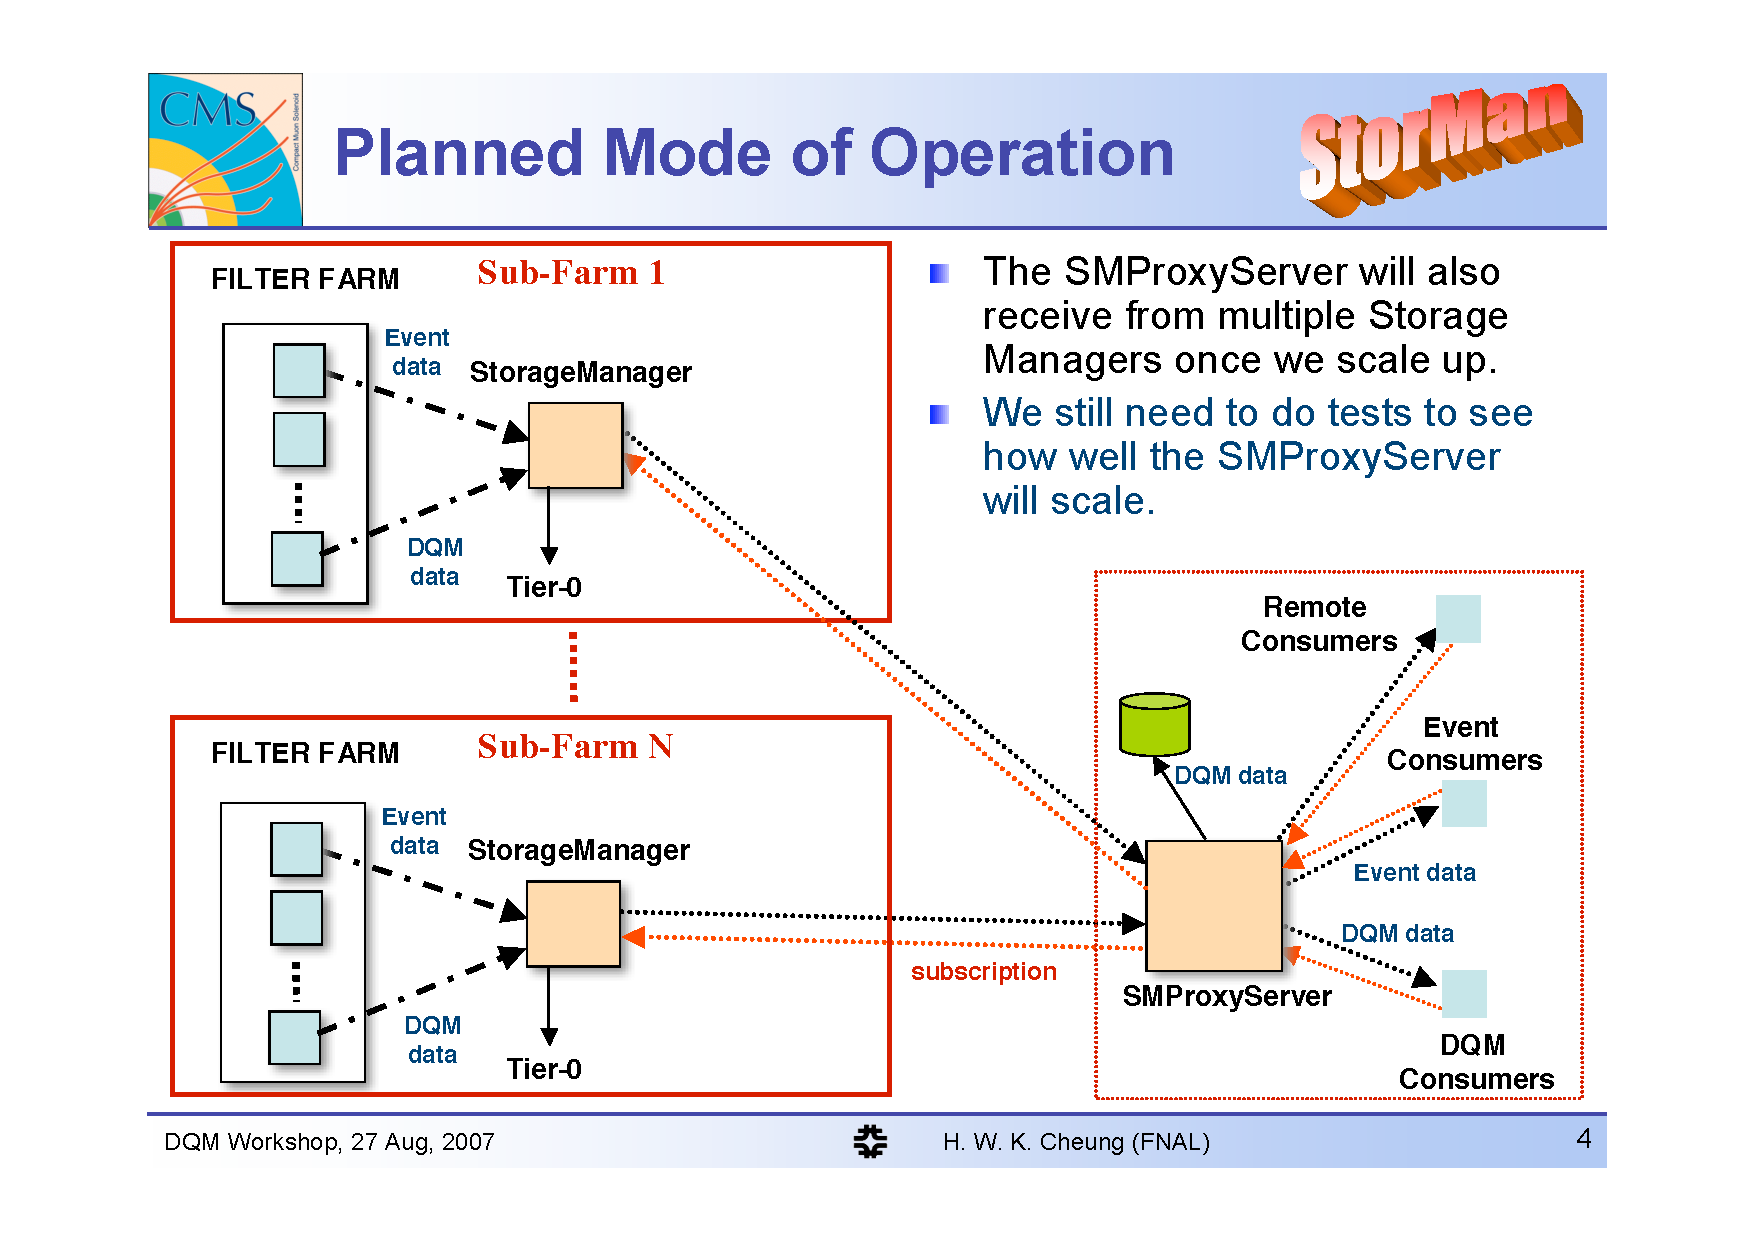
\includegraphics[width=0.9\textwidth]{SM}
\caption{Storage Manager Event and DQM-ME Server 
(figure taken from \cite{talk:harry}).}
\end{center}
\label{fig:sm}
\end{figure}

Fig.~\ref{fig:overview} shows a sketch of the baseline design of the architecture for data quality monitoring using events served by the Storage Manager event server. Several DQM source-client processes (typically one per subsystem) retrieve events through http-request from the event server. The ME (including environmental information, e.g. the runnumber, as well as reference histograms and results from quality tests) are served to one central DQM GUI for visualisation. Alarm states, based on quality test results are also served to the same central display.

\begin{figure}[!htbp]
\begin{center}
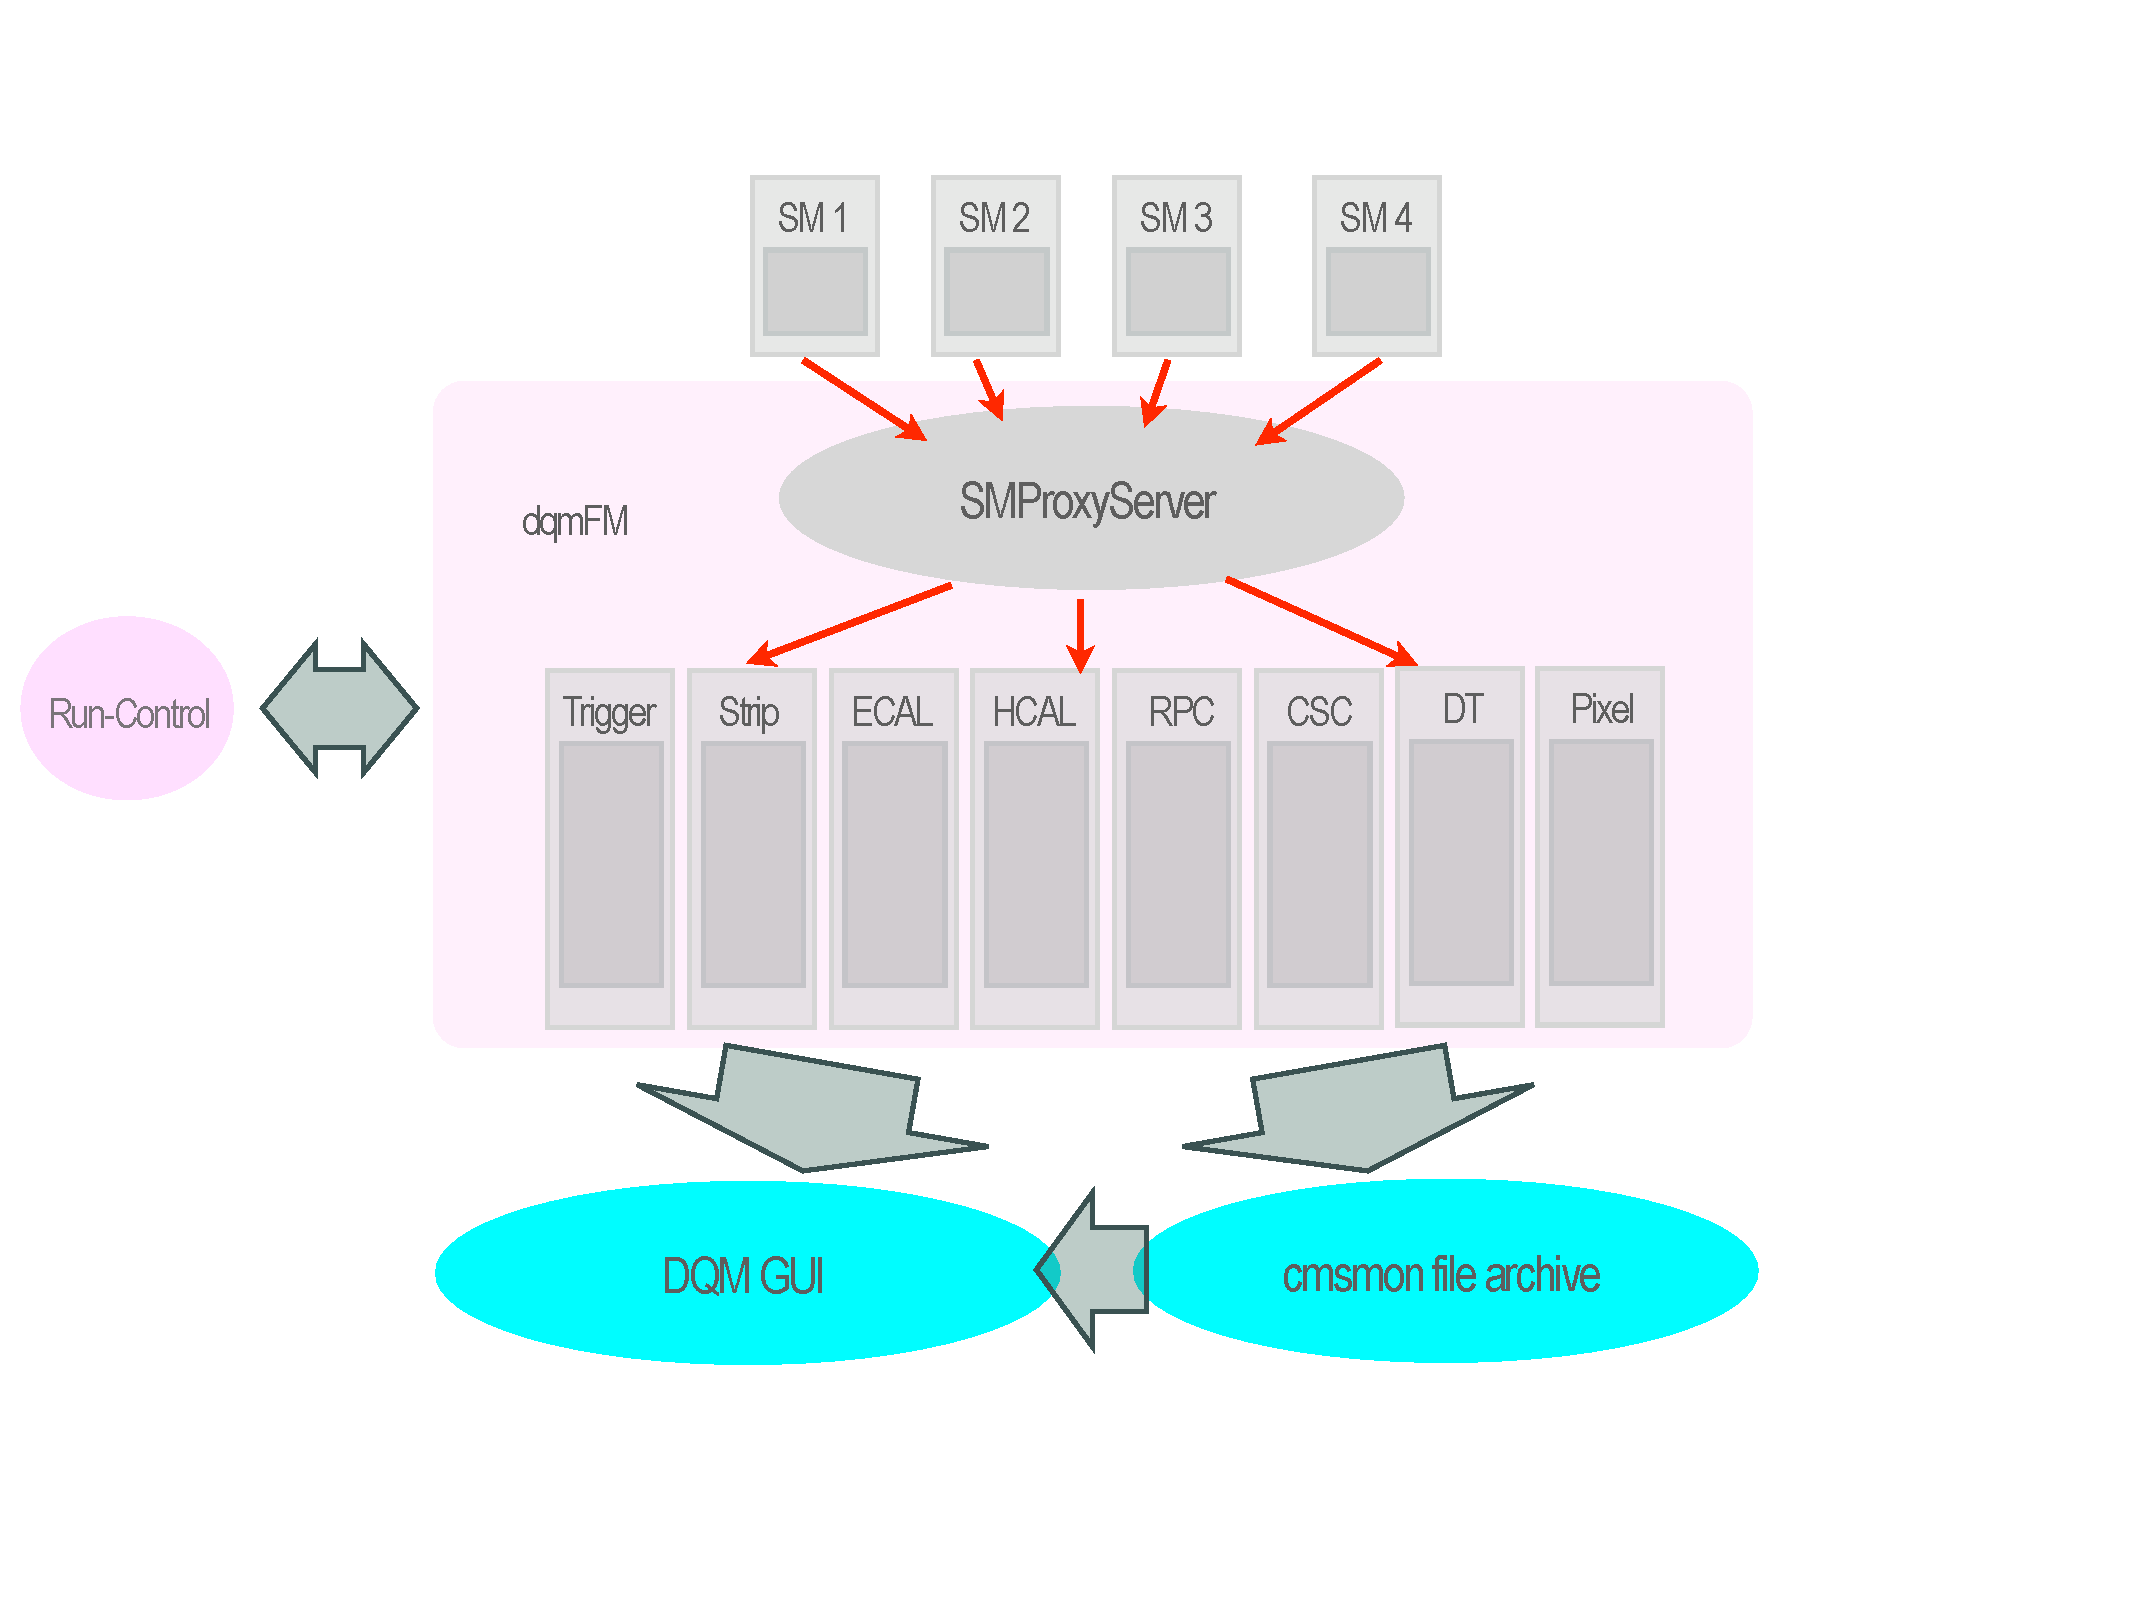
\includegraphics[width=0.9\textwidth]{dqm_online}
\caption{Sketch of the baseline online DQM system.}
\end{center}
\label{fig:overview}
\end{figure}


\subsection{Online DQM Applications}

Event consumer applications are operated on the DQM stream and select events based on trigger paths. The SMProxyServer baseline design foresees no special handling or sorting of events. There will be no provision for parallel event consumers to receive always different events.
DQM applications implement EDAnalyzers for histogram creation and filling. The histograms are stored as MonitorElements and registered to the DQMStore service. Qualitytests are accessible through a generic Qualitytests module and configurable through xml. The specification and implementation of the algorithms is responsibility of the detector performance groups. The DPG provide configurations to the DQM group for review. Reviewed configurations are included in central DQM operation.
The DQM online processes, i.e. the SMProxyServer and the DQM applications (as well as the eventdisplay) are operated within the CMS run-control framework using the level-one DQM function manager. The DQM GUI webservers are operated separately, outside the run-control system

\subsection{Online DQM Stream HLT Configuration}

The event server will be bound to one particular output module that provides the DQM stream.
The DQM stream is a transient event stream that is configurable on the HLT side where the DQM group will be able to specify what HLT paths are to be output and maybe additional paths of their choice, within the general HLT constraint.
Consumer applications can select among the paths which are selected by the DQM output module.

The baseline for the DQMStream contents (i.e. products) is to provide
just raw-data, and to re-run the reconstructions (as much as necessary)
at the DQM consumer level. Additional HLT information can be provided
on request by the consumer application responsible. Optimization of 
event contents, paths and rate sharing is done based on prioritization 
of overall monitoring requirements and bandwidth limitations.
Authoritative priority and optimization decisions are taken based on
discussions within the CMS-wide DQM group.

\subsection{Online DQM Output Archiving and Retrieval}

Each source-client process produces root-file output initially once per run, at the end of a run. 
The root-files are archived in a disk-based spool-area cmsmon.cern.ch.
Several root-files are concatenated into large files. These large
files are made accessible on the web through the DQM webserver-based 
GUI (section \ref{sec:gui}) and backed up to tape. The file handling,
merging, archival, registration with the webserver and backup to tape
are handled by scripts that are operated from cmsmon.
Specific files in the spool-area can be tagged for the purpose of 
providing reference histograms. 

%==========================================================
% this subsection is common to all sections, please fill in
\subsection{Online DQM Integration and Operation}

\subsubsection*{Integration}

The main orientation of the integration work is the standardization of the DQM processes, i.e. the definition and enforcement of standardized DQM interfaces 
and naming conventions.
A large amount of work is spent supporting and consulting the
subsystem responsibles as well as persons starting to use
DQM tools.

\subsubsection*{Operation}

A skeleton online DQM system has been in operation at P5 since November.
Production-level operation was achieved for a few days in a row during
the global runs. This was made possible through maintenance efforts that would be unsustainable over a larger period of time.
At present the development, deployment and maintenance of the 
online production system requires 1-2 FTE. With additional help 
integration and deployment could be accelerated significantly.
Once production is fully established the amount of work for 
operation and maintenance of the online DQM system is estimated to be at least 
1 FTE.

